\chapter{Documentos y esquem\'aticos del hardware}

\section{Herramientas de diseño}

Para todos los diseños se utilizaron herramientas de software libre. Salvo la antena que se diseñó en Geda, el resto se realizó en KiCad.

\subsection{SBC}
\begin{table}[htbp]
\begin{center}
\begin{tabular}{|l|l|}
\hline
\multicolumn{1}{|c|}{\textbf{Componente}} & \multicolumn{1}{c|}{\textbf{Descripción}} \\ \hline
SBC & Beagleboard  RevC4 \\ \hline
Memoria SD & 4GB SDHC Class 6 SD Card \\ \hline
Cable serial DB9 nulo & DB9F Null Modem (RS-232) (6-ft) \\ \hline
Cable conversor usb–serial & USB to DB9M RS-232 (PL-2302) \\ \hline
Cable USB & USB Mini-A to USB A Female, OTG \\ \hline
Cable USB & USB Mini-B Male to USB A Male \\ \hline
Fuente  & 5VDC/2,5A \\ \hline
\end{tabular}
\end{center}
\caption{}
\label{}
\end{table}


\subsection{VLT - Conversor de Voltajes}
\begin{table}[htbp]
\begin{center}
\begin{tabular}{|l|l|c|c|}
\hline
\multicolumn{1}{|c|}{\textbf{Componente}} & \multicolumn{1}{c|}{\textbf{Descripción}} & \textbf{ Footprint} & \textbf{Valor} \\ \hline
C1 & Polarized Capacitor (Tantal) & 6032[2312] & 10uF, 25V \\ \hline
C2 & Polarized Capacitor (Tantal) & 6032[2312] & 100uF, 6V3 \\ \hline
U4 & Regulador LM1117-3.3 & SOT-223 & 3.3V, 800mA \\ \hline
U1, U2, U3 & Voltage Level Translator & TSSOP20 & - \\ \hline
P1 & RECEPTACLE, 28WAY, 2ROW & SMD  Pitch 2,54 & 28 pines \\ \hline
P2 & RECEPTACLE, 40WAY, 2ROW & SMD  Pitch 2,54 & 40 pines \\ \hline
P1b & HEADER, 28WAY, 2ROW & T H Pitch 2,54 & 28 pines \\ \hline
P2b & HEADER, 40WAY, 2ROW & T H Pitch 2,54 & 40 pines \\ \hline
\end{tabular}
\end{center}
\caption{}
\label{}
\end{table}

%\newpage
%\begin{figure}[H]
%\centering
%  \begin{center}
  \includepdf[landscape=true]{pdf/vlt.pdf}
%  \end{center}
%  \caption{VLT - Voltage Level Translator}\label{Fig:HW} 
%\end{figure}
%\newpage

\subsection{SCUI - Lector de tarjetas de contacto e Interfaz de Usuario}
\begin{table}[htbp]
\begin{center}
\begin{tabular}{|l|l|c|c|}
\hline
\multicolumn{1}{|c|}{\textbf{Componente}} & \multicolumn{1}{c|}{\textbf{Descripción}} & \textbf{ Footprint} & \textbf{Valor} \\ \hline
R9 & Resistor 100W 1/4W 1\%  & 3216[1206] & 100W 1/4W  1\% \\ \hline
R10, R13 & Resistor 100KW 1/4W 5\%  & 3216[1206] & 100KW 1/4W   5\% \\ \hline
R11, R12, R14 & Resistor 10KW 1/4W 5\%  & 3216[1206] & 10KW 1/4W   5\% \\ \hline
Q2 & TRANSISTOR, NPN, 300MHZ & SOT23 & MMBT3904 \\ \hline
Q3 & TRANSISTOR, PNP, 250MHZ & SOT23 & MMBT3906 \\ \hline
J2 & SIM socket (6 contacts) & SMD & - \\ \hline
JP3, JP4 & HEADER, 1ROW, 3WAY & T H Pitch 2,54 & 3 pines \\ \hline
X1 & Oscillator 3.579545MHz & SMD & 3.579545 Mhz \\ \hline
ESD1 & Anti ESD & SOT323 & 6V / 150W \\ \hline
\end{tabular}
\end{center}
\caption{}
\label{}
\end{table}

\begin{table}[tbp]
\begin{center}
\begin{tabular}{|l|l|c|c|}
\hline
\multicolumn{1}{|c|}{\textbf{Componente}} & \multicolumn{1}{c|}{\textbf{Descripción}} & \textbf{ Footprint} & \textbf{Valor} \\ \hline
R1 & Resistor 4K7    1/10W     1\% & 1608[0603] & 4,7KW  1/10W   1\% \\ \hline
R2, R8 & Resistor 3R3    1/10W     1\% & 1608[0603] & 3,3W    1/10W   1\% \\ \hline
R3, R4, R5 & Resistor 680R  1/10W     1\% & 1609[0603] & 680W   1/10W   1\% \\ \hline
R6, R7 & Resistor 10K    1/10W     1\% & 1608[0603] & 10KW  1/10W   1\% \\ \hline
RV1 & Preset 15K        1/10W  25\% & SMD & 15KW   1/10W  25\% \\ \hline
Q1 & TRANSISTOR, NPN, 300MHZ & SOT23 & MMBT3904 \\ \hline
S1 & LCD MODULE 16X2 CHARACTER & Pitch 2,54 & - \\ \hline
CONN1 & HEADER FEMALE 16POS.1" TIN & Through Hole & 16 pines \\ \hline
CONN2 & HEADER, 1ROW, 16WAY & T H Pitch 2,54 & 16 pines \\ \hline
LED1 & Led green 5mm & Through Hole & 1,9V,  2mA \\ \hline
LED2 & Led red 5mm & Through Hole & 1,9V,  2mA \\ \hline
LED3 & Led yellow 5mm & Through Hole & 2,4V,  2mA \\ \hline
BUZZ1 & Buzzer & Through Hole & 3~20Vdc, 3~16mA \\ \hline
\end{tabular}
\end{center}
\caption{}
\label{}
\end{table}

%\newpage
%\begin{figure}[H]
%\centering
%  \begin{center}
  \includepdf[landscape=true]{pdf/scui.pdf}
%  \end{center}
%  \caption{SCUI}\label{Fig:HW} 
%\end{figure}
%\newpage
%
%\begin{figure}[H]
%\centering
%  \begin{center}
  \includepdf[landscape=true]{pdf/scui-lector_smart_card.pdf}
%  \end{center}
%  \caption{VLT - Voltage Level Translator}\label{Fig:HW} 
%\end{figure}
%\newpage
%\begin{figure}[H]
%\centering
%  \begin{center}
  \includepdf[landscape=true]{pdf/scui-interfaz_para_usuario.pdf}
%  \end{center}
%  \caption{VLT - Voltage Level Translator}\label{Fig:HW} 
%\end{figure}
%\newpage


\subsection{Lector-Escritor RFID}
\begin{table}[htbp]
\begin{center}
\begin{tabular}{|l|l|c|c|}
\hline
\multicolumn{1}{|c|}{\textbf{Inductor + adaptación}} & \multicolumn{1}{c|}{\textbf{}} & \textbf{} & \textbf{} \\ \hline
\multicolumn{1}{|c|}{\textbf{Componente}} & \multicolumn{1}{c|}{\textbf{Descripción}} & \textbf{ Footprint} & \textbf{Valor} \\ \hline
C1, C2 & Capacitor & 1608[0603] & 10pF,   Ceramic NPO, 2\% \\ \hline
C3, C4 & Capacitor & 1609[0603] & 100pF, Ceramic NPO, 2\% \\ \hline
C5, C6, C7, C8 & Capacitor & 1608[0603] &  NC \\ \hline
R1,  R2 & Resistor & 1608[0603] & 0W,  1/10W,  1\% \\ \hline
\end{tabular}
\end{center}
\caption{}
\label{}
\end{table}

\begin{table}[htbp]
\begin{center}
\begin{tabular}{|l|p{3cm}|c|c|}
\hline
\multicolumn{1}{|c|}{\textbf{CL RC632 + filtro EMC}} &  &  &  \\ \hline
\multicolumn{1}{|c|}{\textbf{Componente}} & \multicolumn{1}{c|}{\textbf{Descripción}} & \textbf{ Footprint} & \textbf{Valor} \\ \hline
C10 & Capacitor & 1610[0603] & 10pF, Ceramic NPO, 2\% \\ \hline
C1, C2 & Capacitor & 1608[0603] & 15pF, Ceramic NPO, 5\% \\ \hline
C12, C13 & Capacitor & 1608[0603] & 56pF, Ceramic NPO, 2\% \\ \hline
C14, C15 & Capacitor & 1608[0603] & 68pF, Ceramic NPO, 1\% \\ \hline
C9 & Capacitor & 1609[0603] & 100pF, Ceramic NPO,  2\% \\ \hline
C16 & Capacitor & 1608[0603] & 1nF, Ceramic NPO, 10\% \\ \hline
C4, C5, C7, C8, C11, C17 & Capacitor & 1608[0603] & 100nF, Ceramic X7R, 10\% \\ \hline
C3, C6, C18 & Capacitor & 1608[0603] & 10uF, Ceramic X5R, 20\% \\ \hline
L1, L2, L3, L6 & Inductor & 2012[0805] & 22nH, 700mA, 5\% \\ \hline
L4, L5 & Inductor & 3225[1210] & 1uH, 400mA, 5\% \\ \hline
R3 & Resistor & 1608[0603] & 50W, 1/10W   1\% \\ \hline
R2 & Resistor & 1608[0603] & 820W, 1/10W   5\% \\ \hline
R1 & Resistor & 1608[0603] & 2,2KW, 1/5W   1\% \\ \hline
U1 & Reader ISO14443 & SO32 & CL RC632 \\ \hline
U2 & Crystal Oscillator, HC49 US SMD & 49USMXL & 13.56MHz, 10pF \\ \hline
U3 & Operational Amplifier (up to 7.5V) & SOT23-5 & OPA354 \\ \hline
CONN1, CONN2 & U.FL-R Connector & U.FL-R-SMT & - \\ \hline
J1 & HEADER, 10WAY, 2ROW & T H Pitch 2,54 & 10 pines \\ \hline
J1b & RECEPTACLE, 10WAY, 2ROW & SMD  Pitch 2,54 & 10 pines \\ \hline
\end{tabular}
\end{center}
\caption{}
\label{}
\end{table}

%\newpage
%\begin{figure}[H]
%\centering
%  \begin{center}
  \includepdf[landscape=true]{pdf/rfid_rwd.pdf}
  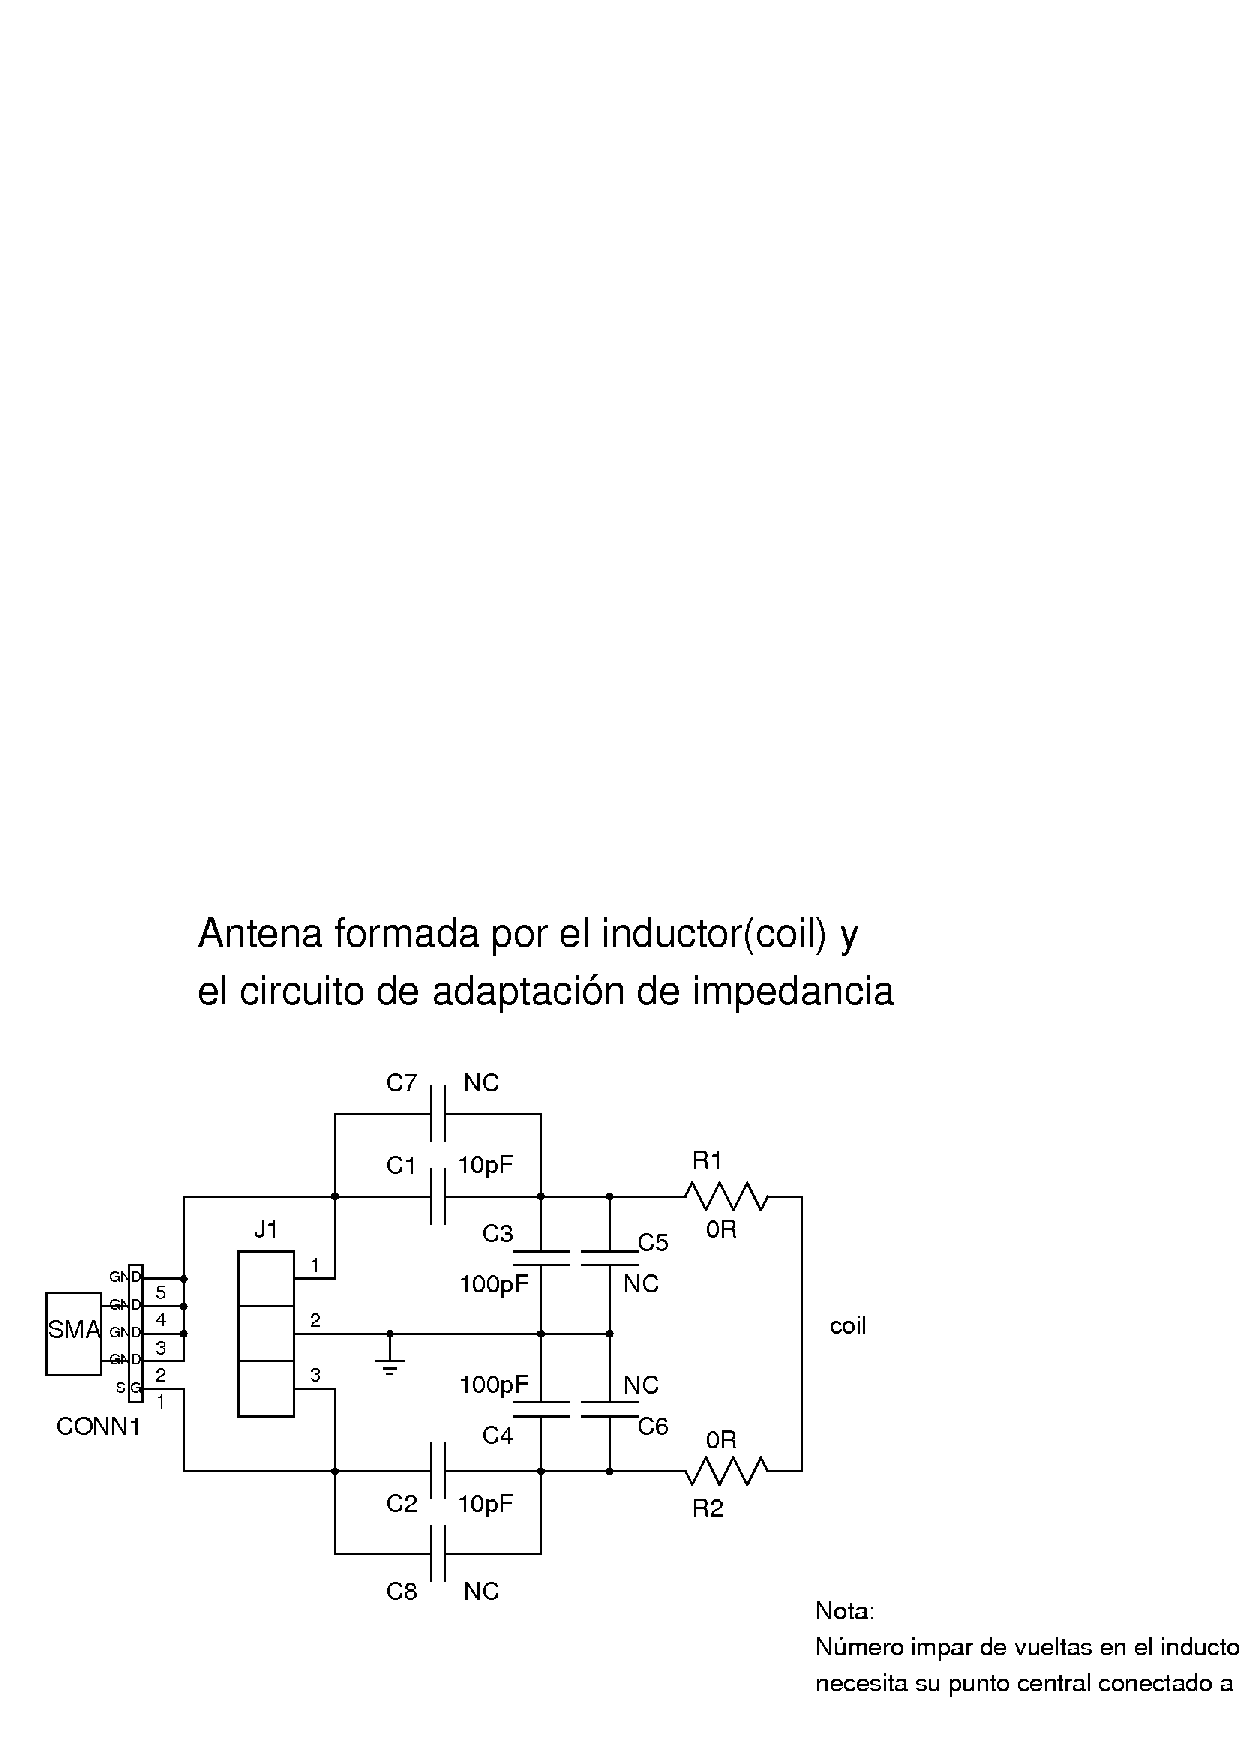
\includepdf[landscape=true]{pdf/rfid_coil.pdf}
%  \end{center}
%  \caption{rfid coil}\label{Fig:HW} 
%\end{figure}
%\newpage

